\graphicspath{{fig/circ_stats_intro/}}

\chapter{Directional statistics}	
\label{cha:direct_stats}

Circular data arises naturally in the study of collective behaviour; most commonly, in
describing the direction of motion of individuals. Given some dataset, the first
instinct of the scientist is to summarise and visualise the data. However, such a
researcher should proceed with caution: circular data cannot be treated as if it were
its linear counterpart.

In this appendix we shall consider why standard techniques, methods and summaries are
inappropriate to use with circular data. After this realisation, we proceed to introduce
some useful techniques which can be used to handle and visualise directional data.

\section{Conventions}
\label{sec:conventions}

Directions can be represented as rotations with respect to some zero-direction, or
origin. The practitioner is free to chose the zero-direction as they feel appropriate. In
a similar way, the practitioner may choose whether a clockwise or anti-clockwise rotation
is taken as the positive direction.

Recall that angles may be represented in units of degrees or radians. To convert between
degrees and radians we may multiply by a factor of $\pi/\ang{180}$.

In this thesis we define the zero-direction as the direction from the point $(0, 0)$ along
the positive $x$-axis. For the most part, we shall measure angles in units of radians, and
take anti-clockwise rotations as the positive direction. The schematics of this setup are
illustrated in \cref{subfig:radian_axes}. Occasionally, we shall appeal to degrees and
their comparative intuitiveness, and in these cases we shall use the setup illustrated in
\cref{subfig:degree_axes}.

\begin{figure}[tb]
\centering
	\begin{subfigure}[b]{0.5\textwidth}
		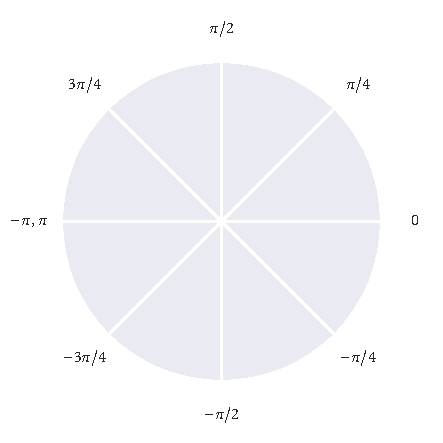
\includegraphics{radian_axes.pdf}
		\caption{}
		\label{subfig:radian_axes}
	\end{subfigure}%
	\begin{subfigure}[b]{0.5\textwidth}
		\centering
		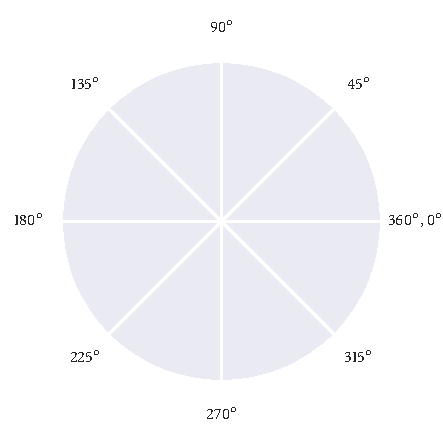
\includegraphics{degree_axes.pdf}
		\caption{}
		\label{subfig:degree_axes}
	\end{subfigure}
    \caption{Visualising the conventions used in this thesis to measure
        \subref{subfig:radian_axes}: radians and \subref{subfig:degree_axes}: degrees.}
	\label{fig:compare_axes}
\end{figure}

\section{Visualisation}
\label{sec:circular_visualisation}

In possession of a dataset, one of the first instincts of the scientist is to visualise
their data. The researcher is undoubtedly familiar with a large number of graph types.
Yet choosing the most suitable graph to display a given dataset is crucial in making an
informative plot.

Traditional histograms are not very good for visualising directional data; consider, for
example, interpreting the directions plotted in \cref{fig:angle_hist}. Polar histograms
(sometimes known as rose plots) make for more intuitive representations of angles.
Instead of using bars, as the histogram does, the rose plot bins data into sectors of a
circle. Here, the \emph{area} of each sector is constructed to be proportional to the
frequency of data points in the corresponding bin \parencite{mardia09}.

\begin{figure}[tb]
	\begin{subfigure}[b]{0.5\textwidth}
		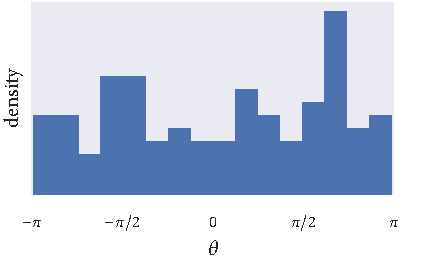
\includegraphics{unif_angle_hist.pdf}
		\caption{}
		\label{subfig:unif_angle_hist}
	\end{subfigure}%
	\begin{subfigure}[b]{0.5\textwidth}
		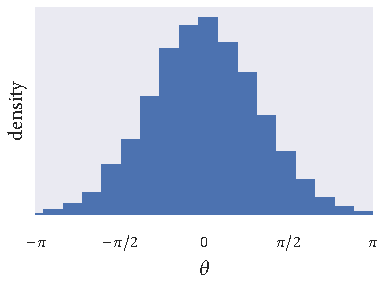
\includegraphics{norm_angle_hist.pdf}
		\caption{}
		\label{subfig:norm_angle_hist}
	\end{subfigure}
    \caption{Using histograms to visualise \subref{subfig:unif_angle_hist}: one hundred
    samples drawn from $U(-\pi, \pi)$ and \subref{subfig:norm_angle_hist}: ten thousand
    samples drawn from $N(0, 1)$.}
	\label{fig:angle_hist}
\end{figure}

\begin{figure}[tb]
	\begin{subfigure}[b]{0.45\textwidth}
		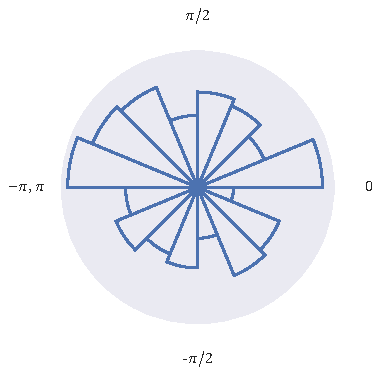
\includegraphics{unif_angle_rose.pdf}
		\caption{}
		\label{subfig:unif_angle_rose}
	\end{subfigure}%
	\hspace{0.05\textwidth}%
	\begin{subfigure}[b]{0.45\textwidth}
		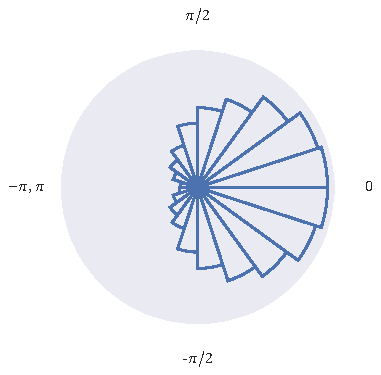
\includegraphics{norm_angle_rose.pdf}
		\caption{}
		\label{subfig:norm_angle_rose}
	\end{subfigure}
    \caption{Using polar histograms to visualise \subref{subfig:unif_angle_hist}: one
    hundred samples drawn from $U(-\pi, \pi)$ and \subref{subfig:norm_angle_hist}: ten
    thousand samples drawn from $N(0, 1)$.}
    \label{fig:angle_rose}
\end{figure}
To advocate the advantages of the rose plot we shall visualise two randomly generated
datasets. The first dataset consists of one hundred realisations from a uniform
$U(-\pi,\pi)$ distribution, and the second dataset consists of ten thousand draws from a
normal $N(0, 1)$ distribution.

In \cref{fig:angle_hist} we visualise the two datasets using traditional histogram plots.
From this figure we get a good idea of the distribution of the data, however we get no
sense of direction.  In \cref{fig:angle_rose} we visualise the same data. Here we also get
a good idea of how the directions are distributed. However, using the rose plot means we
get a very intuitive representation of direction. 

\section{Summary statistics}
\label{sec:summary_stats}

Summary statistics are a useful tool to give an idea of the general characteristics of a
dataset. Probably the first statistic which we learn to compute is the arithmetic mean.
The arithmetic mean, however, is not an appropriate statistic to use with circular data.

Consider that we wish to take an average of the angles $\ang{10}$ and $\ang{350}$. Using
the arithmetic mean we compute an average of $\ang{180}$. However, this average points in
the opposite direction to which we intuitively expect. In \cref{subfig:arith_mean} we
visualise this result.

\begin{figure}
	\begin{subfigure}[b]{0.45\textwidth}
		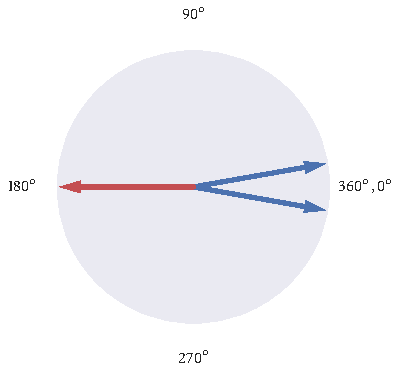
\includegraphics{arith_mean.pdf}
		\caption{Arithmetic mean (red).}
		\label{subfig:arith_mean}
	\end{subfigure}%
	\hspace{0.05\textwidth}
	\begin{subfigure}[b]{0.45\textwidth}
		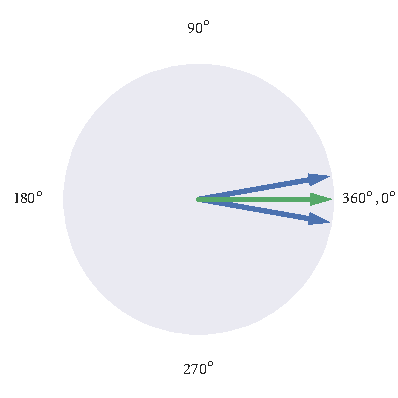
\includegraphics{circ_mean.pdf}
		\caption{Circular mean (green).}
		\label{subfig:circ_mean}
	\end{subfigure}
    \caption{Computing the average of $\ang{10}$ and $\ang{350}$ (represented by the blue
    arrows), using two different mean functions. The green and red arrows show the
    average computed by each method.}
	\label{fig:visualise_mean}
\end{figure}

Before introducing the circular mean it is first necessary to introduce the $\atantwo$
function. The $\atantwo$ function dates back to the Fortran programming language
\parencite{organick66}. It was introduced to overcome some of the inconveniences inherent
in the $\atan$ (or $\tan^{-1}$) function. Consider that the inverse tangent function has
codomain $(-\pi/2, \pi/2)$, though we are often interested in directions in the range
$(-\pi, \pi]$. In addition to this, the $\arctan$ function is not quadrant-aware; that is,
it cannot distinguish between directions which differ by $\pi$ radians (see that
$\tan^{-1}(\theta + \pi) = \tan^{-1}(\theta))$.  As an example,
consider calculating the direction from the $x$-axis to the ray extending from the origin
to the point $(1, 1)$. Naturally, we'd reach for $\tan^{-1}$ to compute the angle as
$\tan^{-1}(1/1) = \pi/4$, as expected. Now, consider that we wish to calculate the
direction from the $x$-axis to the ray extending from the origin to the point $(-1, -1)$.
By inspection, or intuitively, we expect an answer of $-3\pi/4$ --- however, we compute
the answer as $\tan^{-1}(-1/-1) = \pi/4$. The angle calculated using the inverse tangent
function points in the opposite direction to what we expect.

\begin{figure}[tb]
	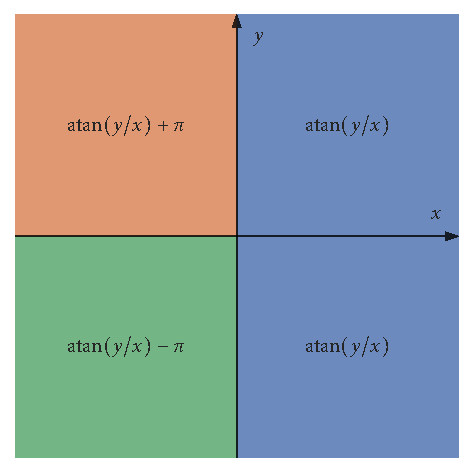
\includegraphics{atan_quadrants.pdf}
	\caption{An illustration of the quadrant corrections made by $\atantwo$.}
	\label{fig:atan_quadrants}
\end{figure}

The $\atantwo$ function, however, does \emph{not} have these shortcomings. The function is
constructed to be quadrant-aware: correcting the computations of $\tan^{-1}$ to return the
directions we intuitively expect. It does so by adding a correction term which depends
on the quadrant which contains our point of interest $(x, y)$. The correction term applied
in each of the four quadrants is visualised in \cref{fig:atan_quadrants}. With these
considerations, $\atantwo$ can be realised by the piecewise function:

\begin{equation}
\label{eq:atantwo}
	\atantwo(y, x) = 
	\begin{cases}
		\atan(y/x)          & \text{ if } x > 0, \\
		\atan(y/x) + \pi    & \text{ if } x < 0 \text{ and } y \geq 0, \\
		\atan(y/x) - \pi    & \text{ if } x < 0 \text{ and } y < 0, \\
		\pi/2               & \text{ if } x = 0 \text{ and } y > 0, \\
		-\pi/2              & \text{ if } x = 0 \text{ and } y < 0, \\
		\text{undefined}    & \text{ if } x = 0 \text{ and } y = 0. \\
	\end{cases}
\end{equation}

As we saw in \cref{subfig:arith_mean}, averaging a set of angles with the arithmetic mean
does not give the desired result. Instead, we must refer to the circular mean. Given a set
of angles $\theta = (\theta_1, \ldots, \theta_n)^T$, we may compute their circular mean
as:
\begin{equation}
	\label{eq:circ_mean}
	\langle \theta \rangle = \atantwo\bigg(\frac{1}{n} \sum_{j=1}^n \sin(\theta_j), \frac{1}{n} 
    \sum_{j=1}^n \cos(\theta_j)\bigg),
\end{equation}
where the $\atantwo$ function is defined in \cref{eq:atantwo} \parencite{fisher95}.

The definition of the circular mean given in equation \cref{eq:circ_mean} works by
converting the angles into Cartesian co-ordinates: representing the directions as points
on the unit circle. The centre of mass of the Cartesian co-ordinates is then computed, and
the resulting position is converted back to a direction, resulting in our mean angle.

In practice, the $1 / n$ which occurs in \cref{eq:circ_mean} is superfluous. Referring to
\cref{eq:atantwo}, see that all of the cases involving $\atan$ require the quotient of $x$
and $y$. Because of this ratio, the $1 / n$ terms will always cancel, and so aren't
strictly necessary.

\section{von Mises distribution}

The von Mises distribution, sometimes simply referred to as the circular normal
distribution, is a continuous probability density function defined on the circle, with
support $[-\pi, \pi)$. The distribution is parameterised by two parameters: $\mu \in
[-\pi, \pi)$ and $\kappa > 0$. The parameter $\mu$ is a measure of location and the
parameter $\kappa$ is a measure of spread. These parameters, $\mu$ and $\kappa$, are
analogous to $\mu$ and $1/\sigma^2$ of the normal distribution.

For the angle $\theta$, the von Mises distribution has probability density:
\begin{equation}
    \label{eq:von_mises}
	f(\theta \given \mu, \kappa) = \frac{e^{\kappa \cos(\theta - \mu)}}%
	                                    {2 \pi I_0(\kappa)},
\end{equation}
where the normalising constant, $I_0(\kappa)$, is the modified Bessel function of the
first kind and order zero \parencite{jammalamadaka01}.

In this thesis we do \emph{not} use the von Mises distribution. Instead, we continue to
use a normal distribution to model circular data. This approximation is
appropriate when $\kappa$ is large (that is, when there is
little dispersion). For large $\kappa$ it is known that $I_0(\kappa) \approx e^k /
\sqrt{2\pi\kappa}$. Using this, and the Taylor expansion $\cos(\alpha) \approx 1 -
\alpha^2/2$, from \cref{eq:von_mises} we have:
\begin{align*}
    f(\theta \given \mu, \kappa) &\approx \frac{e^{\kappa[1-\frac{1}{2}(\theta-\mu)^2]}}%
                                               {2\pi e^k / \sqrt{2\pi\kappa}}\\
                                 & = \frac{e^{-\frac{\kappa}{2}(\theta-\mu)^2}}%
                                          {\sqrt{2\pi/\kappa}},
\end{align*}
which is just the probability density of the normal distribution with mean $\mu$ and precision
$\kappa$. So we see, for distributions with small dispersion, it is appropriate to
approximate the von Mises distribution with a normal distribution.
